% !TeX root = ../../tfg.tex
% !TeX encoding = utf8
%
%*******************************************************
% Construcción y evaluación de las redes neuronales 
%*******************************************************

\chapter{Construcción técnica de las redes neuronales de una sola capa}  

Vista la formulación teórica de una red neuronal de una sola capa 
introducida en \ref{definition:redes_neuronales_una_capa_oculta} explicaremos a continuación  una construcción técnica junto con un
análisis del costo necesario.
 Particularmente el algoritmo presentado es una ligera modificación del algoritmo de    
\textit{forward propagation} explicado en \cite{BishopPaterRecognition}, ha sido necesaria su modificación para ser totalmente fieles a nuestro enfoque teórico. 

Además, puesto que nuestro objetivo es optimizar seremos muy meticulosos en cuanto a analizar el coste computacional tanto de cómputo como de memoria.

\section{Componentes de una red neuronal de una capa oculta} 

Como ya habíamos definido en \ref{definition:redes_neuronales_una_capa_oculta}  
para nosotros una red neuronal será  una función $h : X \longrightarrow Y$ don $X \subseteq \R^d, Y \subseteq \R^s$ 
cuya proyección $k-$ésima viene dada por
\begin{equation}
    h_k(x) =  \sum_{i=1}^{n} \beta_{i k} \gamma_{i}( A_{i}(x))
    = 
    \sum_{i=1}^{n} \beta_{i k} \gamma_{i}
    \left(
        w_{0 i} + \sum_{j=1}^d w_{j i } x_i
    \right) 
\end{equation}
donde $n$ es el número de neuronas,   $\gamma_{i} \in \Gamma$, funciones medibles definidas de $\R$ a $\R$, una red neuronal será 
$\beta_{i k} \in \R$ y $A_i \in \afines$.

% Imagen grafo red neuronal  una capa oculta muy simple y en blanco y negro 
\begin{figure}[h!]
    \centering
    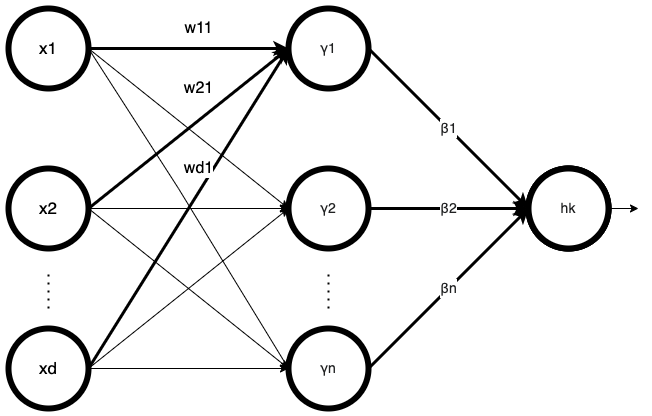
\includegraphics[width=0.85\textwidth]{1-Introduccion_redes_neuronales/Red-Neuronal-una-capa-simple.png}
    \caption{\textit{Grafo} de una red neuronal de una capa oculta}
    \label{img:grafo-red-neuronal-una-capa-oculta_repeticion}
\end{figure}

Analizaremos más a fondo su componentes. 

\subsection*{Construcción de la primera capa}
La primera capa está compuesta por el conjunto de $n$ combinaciones
lineales del vector de entrada $(x_1, \ldots, x_d)$
a las cuales denominaremos \textit{activaciones}, $M$ coincide además
con el número de neuronas en la capa oculta. 

\begin{equation}
    a_i = w_{0 i} + \sum_{i=j}^d w_{j i} x_j 
    \text{ con } j \in \{1, \ldots, n \}.
\end{equation}

Nos referiremos a los  parámetros $w_{j i}$ como 
\textit{pesos} y al parámetro $w_{0 i}$ como 
\textit{sesgo}.  

La memoria que necesaria será de de $(d+1)n \mathfrak{F}$ 
con el $\mathfrak{F}$ la memoria requerida por un peso. 
El coste computacional es además de $d$ multiplicaciones 
y $d+1$ sumas.

\subsection*{Unidades ocultas}
Cada una de esas \textit{activaciones} será transformada
utilizando una \textit{función de activación} $\sigma_j$ 

\begin{equation}
    z_i = \gamma_i(a_i).
\end{equation}
En el contexto de las redes neuronales a $z_i$ se le conoce como \textit{unidad oculta}. Ésta  podría ser de 
nuevo  transformada por una combinación lineal, en nuestro caso tan solo 
por el producto de un escalar, ya que como se adelantó en la sección \ref{subsection:diferencia-otras-definiciones-RRNN},
 frente a la transformación afín usualmente propuesta, esta transformación no es necesaria para asegurar la convergencia, profundizaremos más sobre esto más adelante. 

Finalmente la salida vendrá dada por
 \begin{equation}
    h_k = \sum_{i=1}^n \beta_i z_i 
    \text{ con } i \in \{1, \ldots, s \}.
\end{equation}
Nótese que ahora el tamaño de variables de entrada es $M$
y hay un total de $s$ unidades de activación, tanto $M$ como $s$ son
valores fijados por el diseñador de la red ya que a priori no tenemos otra información. 
 
 % Vamos a probar que tampoco mejora el error 
\subsection{Consideraciones sobre la irrelevancia del sesgo}

 Dados $X \subseteq \R^d, Y \subseteq \R^s$ y  $\Gamma$ un conjunto no vacío de funciones medibles definidas de $\R$ a $\R$, denotaremos como $\mathcal{H}^+(X,Y)$ al conjunto de redes neuronales a las cuales se le ha añadido un sesgo. 

\begin{align}
    \mathcal{H}^+(X,Y) 
    =
    \{
        h : X \longrightarrow Y 
        /& \quad 
        h_k(x) = 
        \sum_{i=1}^{n} \left( \beta_{i k} \gamma_{i}( A_{i}(x)) + \alpha_{i k} \right), \\
        & \text{donde  $h_k$  es la proyección k-ésima de $h$ con 
        $k \in \{1, \ldots, s\}$}, \\
        & n \in \N,\gamma_{i} \in \Gamma , \beta_{i k} \in \R
         \text{ y }A_{i} \text{ una aplicación afín de $\R^d$ a $\R$}           
    \}.
\end{align}


Está claro que al introducir tal sesgo se añade en memoria 
un coste de $n \mathfrak{F}$ con $n$ el número de neuronas en la capa oculta y que además el costo de cómputo se ve aumentado en la misma proporción. 

Sin embargo podría obtenerse un beneficio en cuanto a precisión, 
vamos a proceder  a analizar esta idea. 

Es evidente que 
\begin{equation} \label{eq:conjuntos-redes-neuronales-con-sesgo-contiene-elemental}
    \mathcal{H}(X,Y) \subseteq \mathcal{H}^+(X,Y)
\end{equation}

Además al estar trabajando con una sola capa, se tiene que para cualquier 
$h^+ \in \mathcal{H}^+(X,Y)$

\begin{align}
    h^+ = \sum_{i=1}^{n} \left(\beta_{i k} \gamma_{i}( A_{i}(x)) + \alpha_{i k} \right)
    = \sum_{i=1}^{n} \left(\beta_{i k} \gamma_{i}( A_{i}(x))\right) + k 
\end{align}
Con $k \in \R$ un parámetro libre.

Ante esto, al igual que se hacía en el lema \ref{lema:A_3_función_activación_continua_con_arbitaria}
es fácil obtener una neurona de valor constante y por tanto, para un conjunto fijo de neuronas $n$, se tiene que 
\begin{equation}
    \mathcal{H}^+_n(X,Y) \subsetneq  \mathcal{H}_{n+1}(X,Y),
\end{equation}
de esta relación se obtienen dos cosas: 
puesto que $n$ era arbitrario y 
\begin{equation}
    \mathcal{H}(X,Y) = \bigcup_{n \in \N} \mathcal{H}_n (X,Y)
\end{equation}
entonces como espacios de funciones 
\begin{equation}
    \mathcal{H}(X,Y) = \mathcal{H}^+ (X,Y).
\end{equation}
Por otra parte no hace reparar que la precisión que pueda aportar el sesgo es
superada añadiendo una neurona más a un modelo sin sesgo, es más, también se obtiene una mejora en memoria, ya que 
$\mathcal{H}^+_n(X,Y)$ requiere de $n \mathfrak{F}$ espacio de memoria adicional con respecto a $\mathcal{H}_n(X,Y)$
mientras que $\mathcal{H}_{n+1}(X,Y)$ de $(D +1) \mathfrak{F}$
y por lo visto en el teorema de convergencia universal \ref{teo:MFNAUA}, la precisión se consigue añadiendo neuronas (la dimensión de los datos es fija),
luego podemos suponer que $n$ será mayor que $D+1$. 

Hasta ahora hemos comparado la capacidad de expresión 
por la forma de los elementos de los conjuntos, para comparar su bondad aproximando, vamos a fijar  un 
 número de capas ocultas $n$ y 
 y una función de error cualquiera que mida el error dentro 
 del conjunto de entrenamiento
 $E_{\mathcal{D}}:\mathcal{H}^+(X,Y) \longrightarrow \R^+_0$.
 
 Todas las normas en $\R^n$ son equivalentes luego no hay pérdida de generalidad fijando una cualquiera.  

 Definimos también el error dentro del espacio $\Lambda$ como 
 \begin{equation}
    \mathcal{E}_{\mathcal{D}} (\Lambda)
    = \inf \{ E_{\mathcal{D}}(h) : h \in \Lambda\}.
 \end{equation}

Está claro por la relación  
 (\refeq{eq:conjuntos-redes-neuronales-con-sesgo-contiene-elemental})
 que 
 \begin{equation}
    \mathcal{E}_{\mathcal{D}}(\mathcal{H}^+(X,Y))
    \leq
    \mathcal{E}_{\mathcal{D}}(\mathcal{H}(X,Y))
 \end{equation}

 La clave ahora reside en si se satisface la desigualdad opuesta
Es decir, dada cualquier $h^+ \in \mathcal{H}^+_n(X,Y)$ con un error de $E_D(h^+)$ existe $h \in \mathcal{H}_n(X,Y)$  tal que $E_D(h) \leq E_D(h^+).$  
Esto no es posible para todo los casos, fijamos $h^+ \in \mathcal{H}^+_n(X,Y)$ y tomamos como conjunto de datos $\mathcal{D}$ el grafo de $h^+$, es evidente que $E_{\mathcal{D}}(h^+) = 0$ entonces si existiera $h \in \mathcal{H}_n(X,Y)$ con $E_{\mathcal{D}}(h) \leq E_{\mathcal{D}}(h^+)$ necesariamente $E_{\mathcal{D}}(h) = 0$ y entonces $h^+ \in \mathcal{H}_n(X,Y)$ por lo que se tendría que 
$$\mathcal{H}_n(X,Y) = \mathcal{H}_n^+(X,Y)$$ 
lo cual es una contradicción.

Notemos que en la práctica el conjunto $\mathcal{D}$ es finito, 
por lo que habrá situaciones en que para ese conjunto de datos sí  se tenga la misma precisión. 

% Fin de la demostración 

 Concluimos tras todo esto que aunque la precisión que se pueda obtener con funciones de $\mathcal{H}_n(X,Y)$ y $\mathcal{H}^+_n(X,Y)$ es diferente para un mismo número de neuronas $n$, añadiendo una más el sesgo es irrelevante  y además $\mathcal{H}^+_n(X,Y)$ tiene mayor coste computacional, por lo que afirmamos que 
que es un artificio de las redes neuronales multicapa para enlazar una capa con otra y que en redes neuronales de una capa oculta carece de sentido.

% Consideración sobre componer la red neuronal con una función
\subsection{Consideraciones sobre la composición de redes neuronales con otras funciones}

Es usual en la literatura presentar las redes neuronales con la salida compuesta con una función $\theta$, de tal manera que una red neuronal sea de la forma

\begin{equation}
    h_k(x) = \theta_k 
    \left(
        \sum_{i=1}^{n} \beta_{i k} \gamma_{i}
    \left(
        w_{0 i} + \sum_{j=1}^d w_{j i } x_i
    \right) 
    \right)
    \text{ para cada  } k \in \{1, \ldots, s \}.
\end{equation}
El teorema universal de convergencia \ref{teo:MFNAUA} nos asegura 
que dado un número lo suficientemente grande de neuronas tal 
composición no es necesaria, sin embargo a nivel práctico ese 
número de neuronas puede no alcanzarse y por cómo se produce la convergencia el resultado serán funciones con imágenes contenidas en $\R^n$.

Por la naturaleza de la imagen de ciertos problemas no sería necesaria mayor modificación y con nuestra definición sería más que suficiente, pero en caso de la salida tener que cumplir alguna restricción como  un problema de clasificación que necesite una salida discreta por lo observado en \ref{corolario:2_5_función_Booleana} aunque la convergencia esté asegurada para asegurarnos que se cumplen tales restricciones sería necesario la composición con una función $\theta$.

\textcolor{red}{Pensar en el debate de si entrenar y luego determinar $\theta$ o directamente entrenar con $\theta$ (esto vendrá determinado por el método de aprendizaje que usemos y si $\theta$ se lleva bien con él.)}

%%%%%%%%%%% Fin de lo observado

\subsection{Qué función de activación seleccionar}

Los aspectos a tener en cuenta a la hora de seleccionar una función 
de activación frente a otra de una red neuronal serían los siguientes:
\begin{enumerate}
    \item Espacio de memoria.
    \item Coste computacional.
    \item Precisión a obtener.
\end{enumerate}

Sobre la primera consideración está claro que el uso de una única función ahorraría el tener que almacenar el tipo de función que se va emplear en cada neurona.

Respecto al coste computacional para se han observado los siguientes
\textcolor{red}{TODO:  añadir coste computacional  de las funciones que considere oportunas}

Y respecto a la precisión no se conoce ninguna motivación (por ahora)
que \textcolor{red}{TODO pensar}

\textcolor{red}{TODO: Pudiera existir un equilibrio entre 
el coste y la precisión. Ie, a mismo número de neuronas se podría conseguir mejor precisión con ciertas funciones de activación -> esto seguro. ¿Cómo se podría saber esto a partir de los datos? ¿aumentaría ese proceso el coste?}


%% Formulación técnica 

\section{Explicitación de la construcción de una red neuronal}
